\documentclass[11pt,a4paper]{article}
\usepackage[margin=1in]{geometry}
\usepackage[T1]{fontenc}
\usepackage[utf8]{inputenc}
\usepackage{lmodern}
\usepackage{booktabs}
\usepackage{longtable}
\usepackage{graphicx}
\usepackage{float}
\usepackage{hyperref}
\usepackage{setspace}
\usepackage{enumitem}

\title{Semester Project: Domain Discovery, Recommendation, and Graph Intelligence\\
\large Milestone: Dataset Charter, Processed Dataset V1, and EDA}
\author{Iam Anthony Marcelo Alvarez Orellana \\ Jeffrey Ulises Diaz Villanueva \\ Paula Jimena Mancilla Cienfuegos \\ Fernando Samuel Paredes Espinoza}
\date{}

\begin{document}
\maketitle
\onehalfspacing

\section*{Team 6 Members}
\begin{center}
\begin{tabular}{cl}
\toprule
\textbf{\#} & \textbf{Team Member} \\
\midrule
1 & Iam Anthony Marcelo Alvarez Orellana \\
2 & Jeffrey Ulises Diaz Villanueva \\
3 & Paula Jimena Mancilla Cienfuegos \\
4 & Fernando Samuel Paredes Espinoza \\
\bottomrule
\end{tabular}
\end{center}

\section{Project Proposal}
\begin{itemize}[leftmargin=*]
  \item \textbf{Domain:} Global Digital Video Game Marketplace (Steam).
  \item \textbf{Problem Statement:} With over 80,000 titles available, the Steam platform faces an acute \textbf{"Choice Overload"} problem. Users typically gravitate toward high-budget (AAA) titles, while high-quality niche (Indie) games remain undiscovered. Traditional popularity-based ranking systems fail to capture latent connections between complex gameplay preferences and community-driven structures.
  \item \textbf{Expected Product Question:} How can we improve game discovery through a hybrid system that leverages community-driven tag centrality within a graph and historical user behavior (playtime) to recommend titles with high satisfaction probability?
  \item \textbf{Suitability for the course:} This dataset is ideal for building the four mandatory course layers:
  \begin{itemize}[leftmargin=*]
    \item \textbf{Catalog Layer:} Technical and commercial game metadata (genres, developers, tags).
    \item \textbf{Feature Layer:} Vectorization of game descriptions and community tags for similarity analysis.
    \item \textbf{Interaction Layer:} A dataset of \textasciitilde 480k unique interactions including playtime and voting behavior.
    \item \textbf{Graph Layer:} Bipartite User-Game graphs and Tag-to-Tag co-occurrence networks.
  \end{itemize}
\end{itemize}

\section{Source Inventory}
\begin{itemize}[leftmargin=*]
  \item \textbf{Source URLs:}
  \begin{itemize}[leftmargin=*]
    \item \href{https://www.kaggle.com/datasets/artermiloff/steam-games-dataset}{Steam Games Dataset 2025 - Artemiy Ermilov (Kaggle)}
    \item \href{https://www.kaggle.com/datasets/artermiloff/steam-games-reviews-2024}{Steam Games Reviews 2024/2025 - Artemiy Ermilov (Kaggle)}
  \end{itemize}
  \item \textbf{Licenses:} CC0: Public Domain / Kaggle Dataset Terms of Use.
  \item \textbf{Raw File Formats:} CSV (multiple files for reviews) and a single CSV for the game catalog.
  \item \textbf{Estimated Size:} Approximately 128 million total records in the universe, sampled down for the V1 working subset.
\end{itemize}

\section{Schema Draft}
The system follows a star schema architecture where \texttt{AppID} serves as the central join key between the catalog and the interaction layers.

\begin{itemize}[leftmargin=*]
  \item \textbf{Main Entities:}
  \begin{itemize}[leftmargin=*]
    \item \textbf{Games (Catalog):} Technical, commercial, and descriptive metadata.
    \item \textbf{Reviews (Interactions):} User sentiment, engagement metrics, and behavioral data.
  \end{itemize}
  \item \textbf{Keys:}
  \begin{itemize}[leftmargin=*]
    \item \texttt{AppID}: Primary Key for Games table; Foreign Key for Reviews.
    \item \texttt{author\_steamid}: Unique identifier for users (Author).
    \item \texttt{recommendationid}: Unique identifier for each interaction/review record.
  \end{itemize}
  \item \textbf{Expected Joins:} Inner join on \texttt{AppID} to enrich interaction data with genres, tags, and developer information.
\end{itemize}

\section{Data Dictionary Draft (Core Features)}
\subsection*{Table: Games (Catalog)}
\begin{longtable}{p{0.22\linewidth}p{0.18\linewidth}p{0.52\linewidth}}
\toprule
\textbf{Column} & \textbf{Type} & \textbf{Description} \\
\midrule
\texttt{AppID} & Integer & Unique identifier for the game on the Steam platform. \\
\texttt{name} & String & Official title of the videogame. \\
\texttt{genres} & String & Primary categories (e.g., Action, RPG, Strategy). \\
\texttt{tags} & String & Community-driven descriptors used for graph construction. \\
\texttt{price} & Float & Current retail price in USD. \\
\texttt{average\_playtime\_forever} & Integer & Average playtime across all owners (global baseline). \\
\bottomrule
\end{longtable}

\subsection*{Table: Reviews (Interactions)}
\begin{longtable}{p{0.22\linewidth}p{0.18\linewidth}p{0.52\linewidth}}
\toprule
\textbf{Column} & \textbf{Type} & \textbf{Description} \\
\midrule
\texttt{recommendationid} & Integer & Unique ID for the specific review record. \\
\texttt{author\_steamid} & String & Anonymized unique ID of the user. \\
\texttt{voted\_up} & Boolean & Target variable: indicates if the user recommends the game. \\
\texttt{author\_playtime\_forever} & Float & Total hours played by the specific user (engagement metric). \\
\texttt{author\_num\_games\_owned} & Integer & User profile feature representing library depth. \\
\bottomrule
\end{longtable}

\section{Scale Analysis (V1)}
\begin{itemize}[leftmargin=*]
  \item \textbf{Total Raw Files Found:} 79,994 files.
  \item \textbf{V1 Working Subset:} 500 game files processed.
  \item \textbf{Rows in V1:} 480,025 unique interaction records.
  \item \textbf{Columns:} 67 original columns reduced to 12 prioritized features in the pipeline.
  \item \textbf{Sparsity Estimate:} \textasciitilde 99.8\% (standard for large-scale recommendation domains).
  \item \textbf{Memory Footprint:} \textasciitilde 115 MB in optimized Parquet format.
\end{itemize}

\section{Ethics and Access Note}
\begin{itemize}[leftmargin=*]
  \item \textbf{Provenance:} Data is sourced from the public Steamworks API and structured by researchers for academic purposes.
  \item \textbf{Authorization:} Data use is permitted under the Steam API Terms of Service for research and non-commercial development.
  \item \textbf{Personal Data Risks:} The dataset includes \texttt{author\_steamid}. While these are public profiles, there is a risk of profile tracking.
  \item \textbf{Risk Mitigation:} The ingestion pipeline excludes free-text comments to prevent PII leakage. IDs are treated as opaque numerical identifiers. No emails, real names, or financial data are collected or stored.
\end{itemize}

\section{Technical Expectation: Ingestion Command}
To reproduce the processed V1 dataset, run the following command from the project root:

\begin{verbatim}
# 1. Activate virtual environment
# Windows: .\venv\Scripts\activate | Mac/Linux: source venv/bin/activate

# 2. Run ingestion pipeline
python src/ingest.py
\end{verbatim}

\section{Exploratory Data Analysis (EDA)}
The EDA was generated from \texttt{data/processed/steam\_v1.parquet}. Figures are exported as PNG files and included below.

\noindent\textbf{Important methodological note.} This report is based on the V1 subset (500 review files), not the full universe of available Steam review files. Therefore, absolute counts and ranking positions can vary across runs depending on which files are included in the subset and how source files are discovered in the file system. The plots should be interpreted as an initial analytical baseline for pattern discovery, not as final population-level estimates.

\subsection*{1) Recommendations Distribution}
This chart summarizes the class balance of user sentiment (recommended vs not recommended). In our sample, positive recommendations dominate, which is a common behavior in review ecosystems. Even if exact counts change with a different subset, this figure is useful to assess target imbalance before modeling and to plan metrics beyond raw accuracy.

\begin{figure}[H]
  \centering
  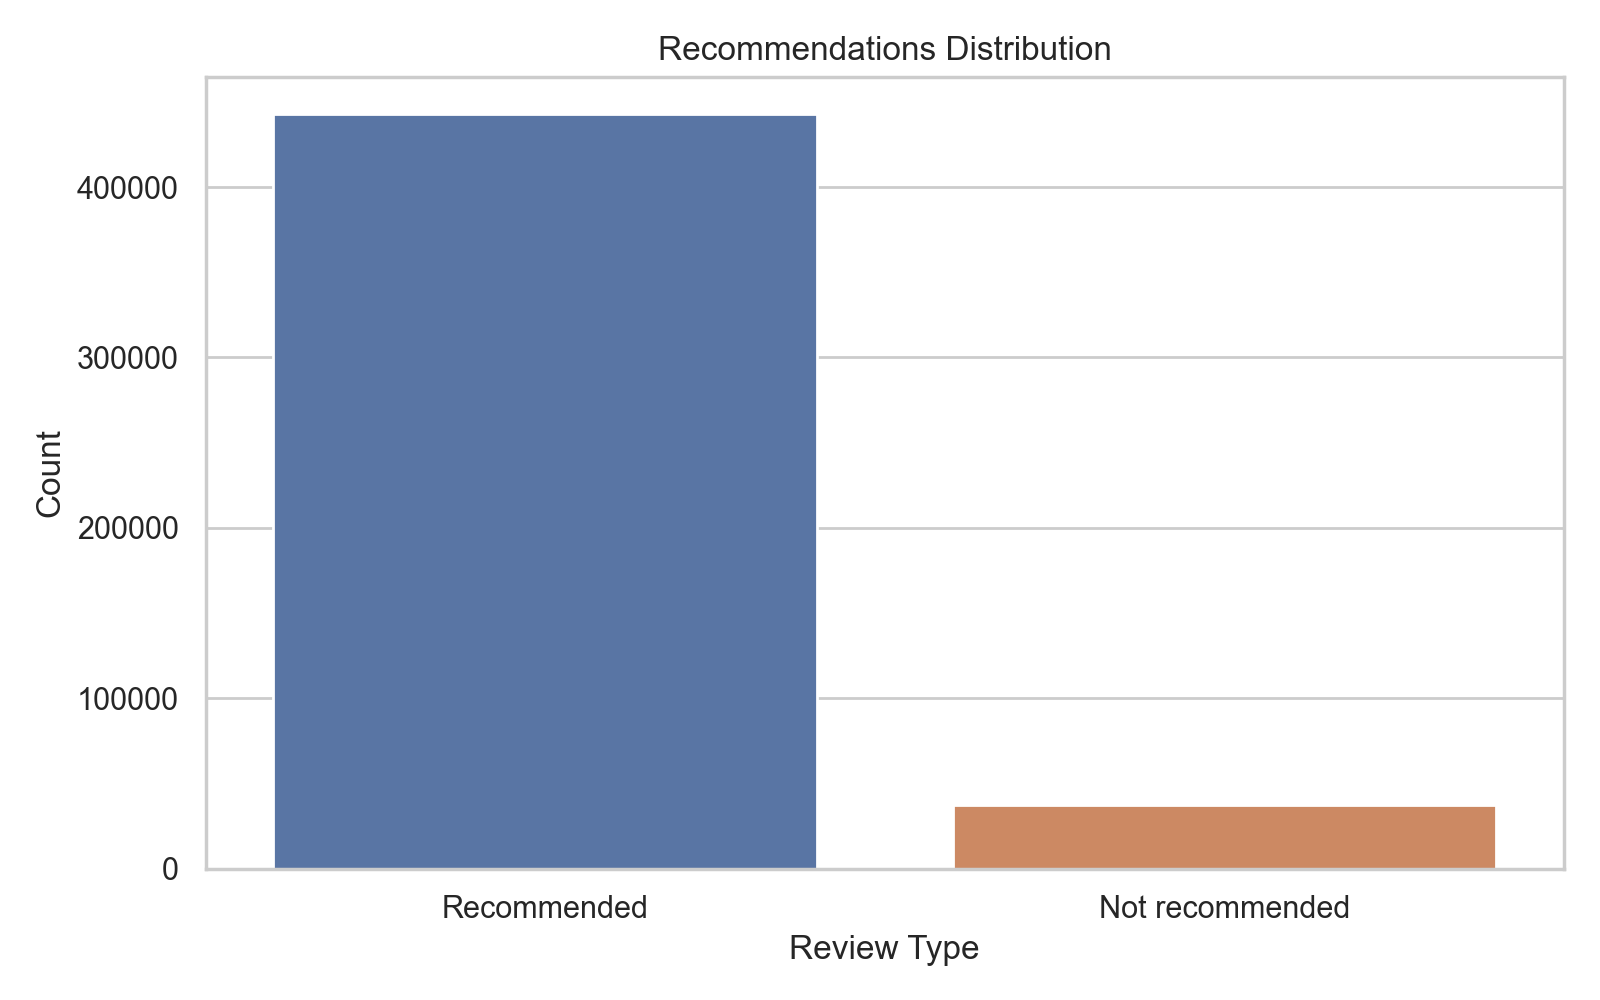
\includegraphics[width=0.85\linewidth]{eda/01_recommendations_distribution.png}
  \caption{Distribution of recommendation labels (Recommended vs Not recommended).}
\end{figure}

\subsection*{2) Playtime Distribution}
This histogram shows strong right skew: most users accumulate relatively low-to-moderate playtime, while a smaller group contributes very high values. The 99th-percentile cap improves readability and prevents outliers from compressing the main body of the distribution. The exact tail magnitude may vary with sample composition, but the skewed shape is typically stable.

\begin{figure}[H]
  \centering
  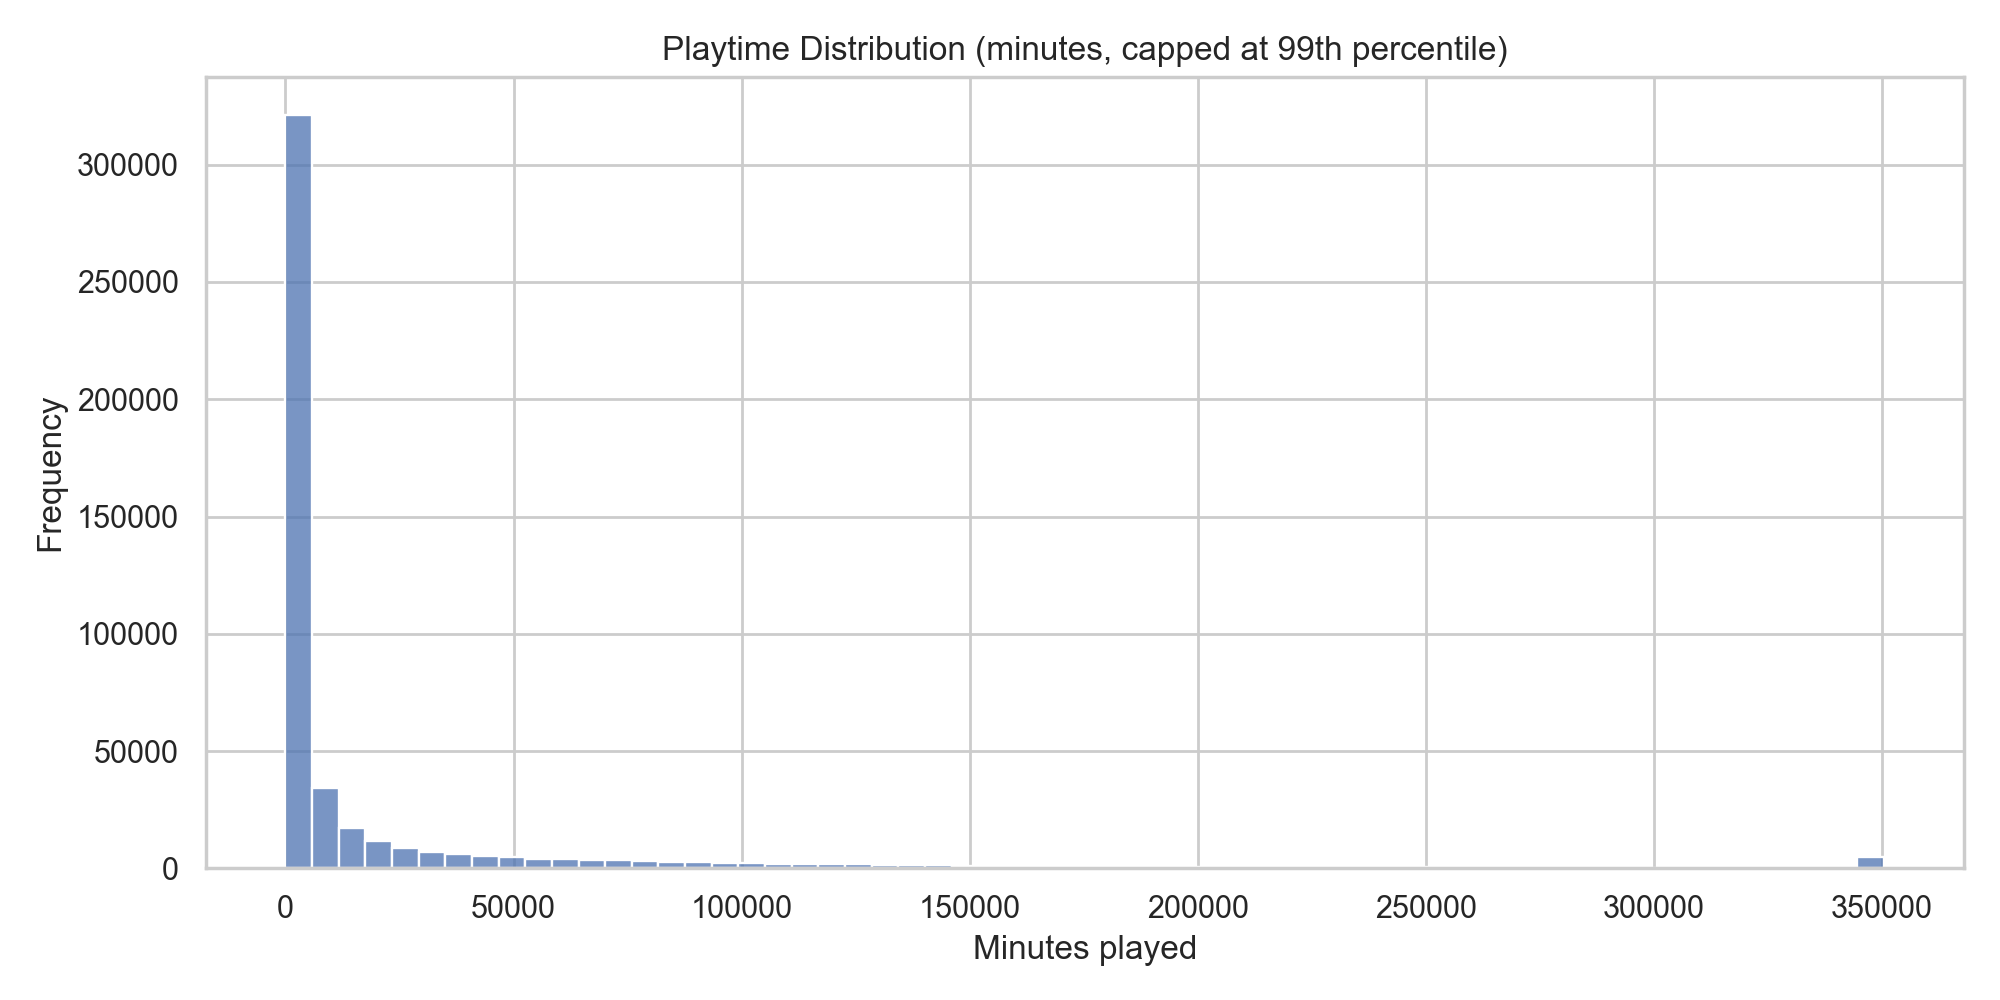
\includegraphics[width=0.9\linewidth]{eda/02_playtime_distribution.png}
  \caption{Playtime distribution in minutes, capped at the 99th percentile for readability.}
\end{figure}

\subsection*{3) Top Games by Review Volume}
This ranking identifies which titles concentrate the largest number of interactions in the working subset. It is useful for understanding exposure concentration and potential popularity bias in downstream recommenders. Since this is subset-based, specific game order can shift between runs, but the long-tail structure usually remains.

\begin{figure}[H]
  \centering
  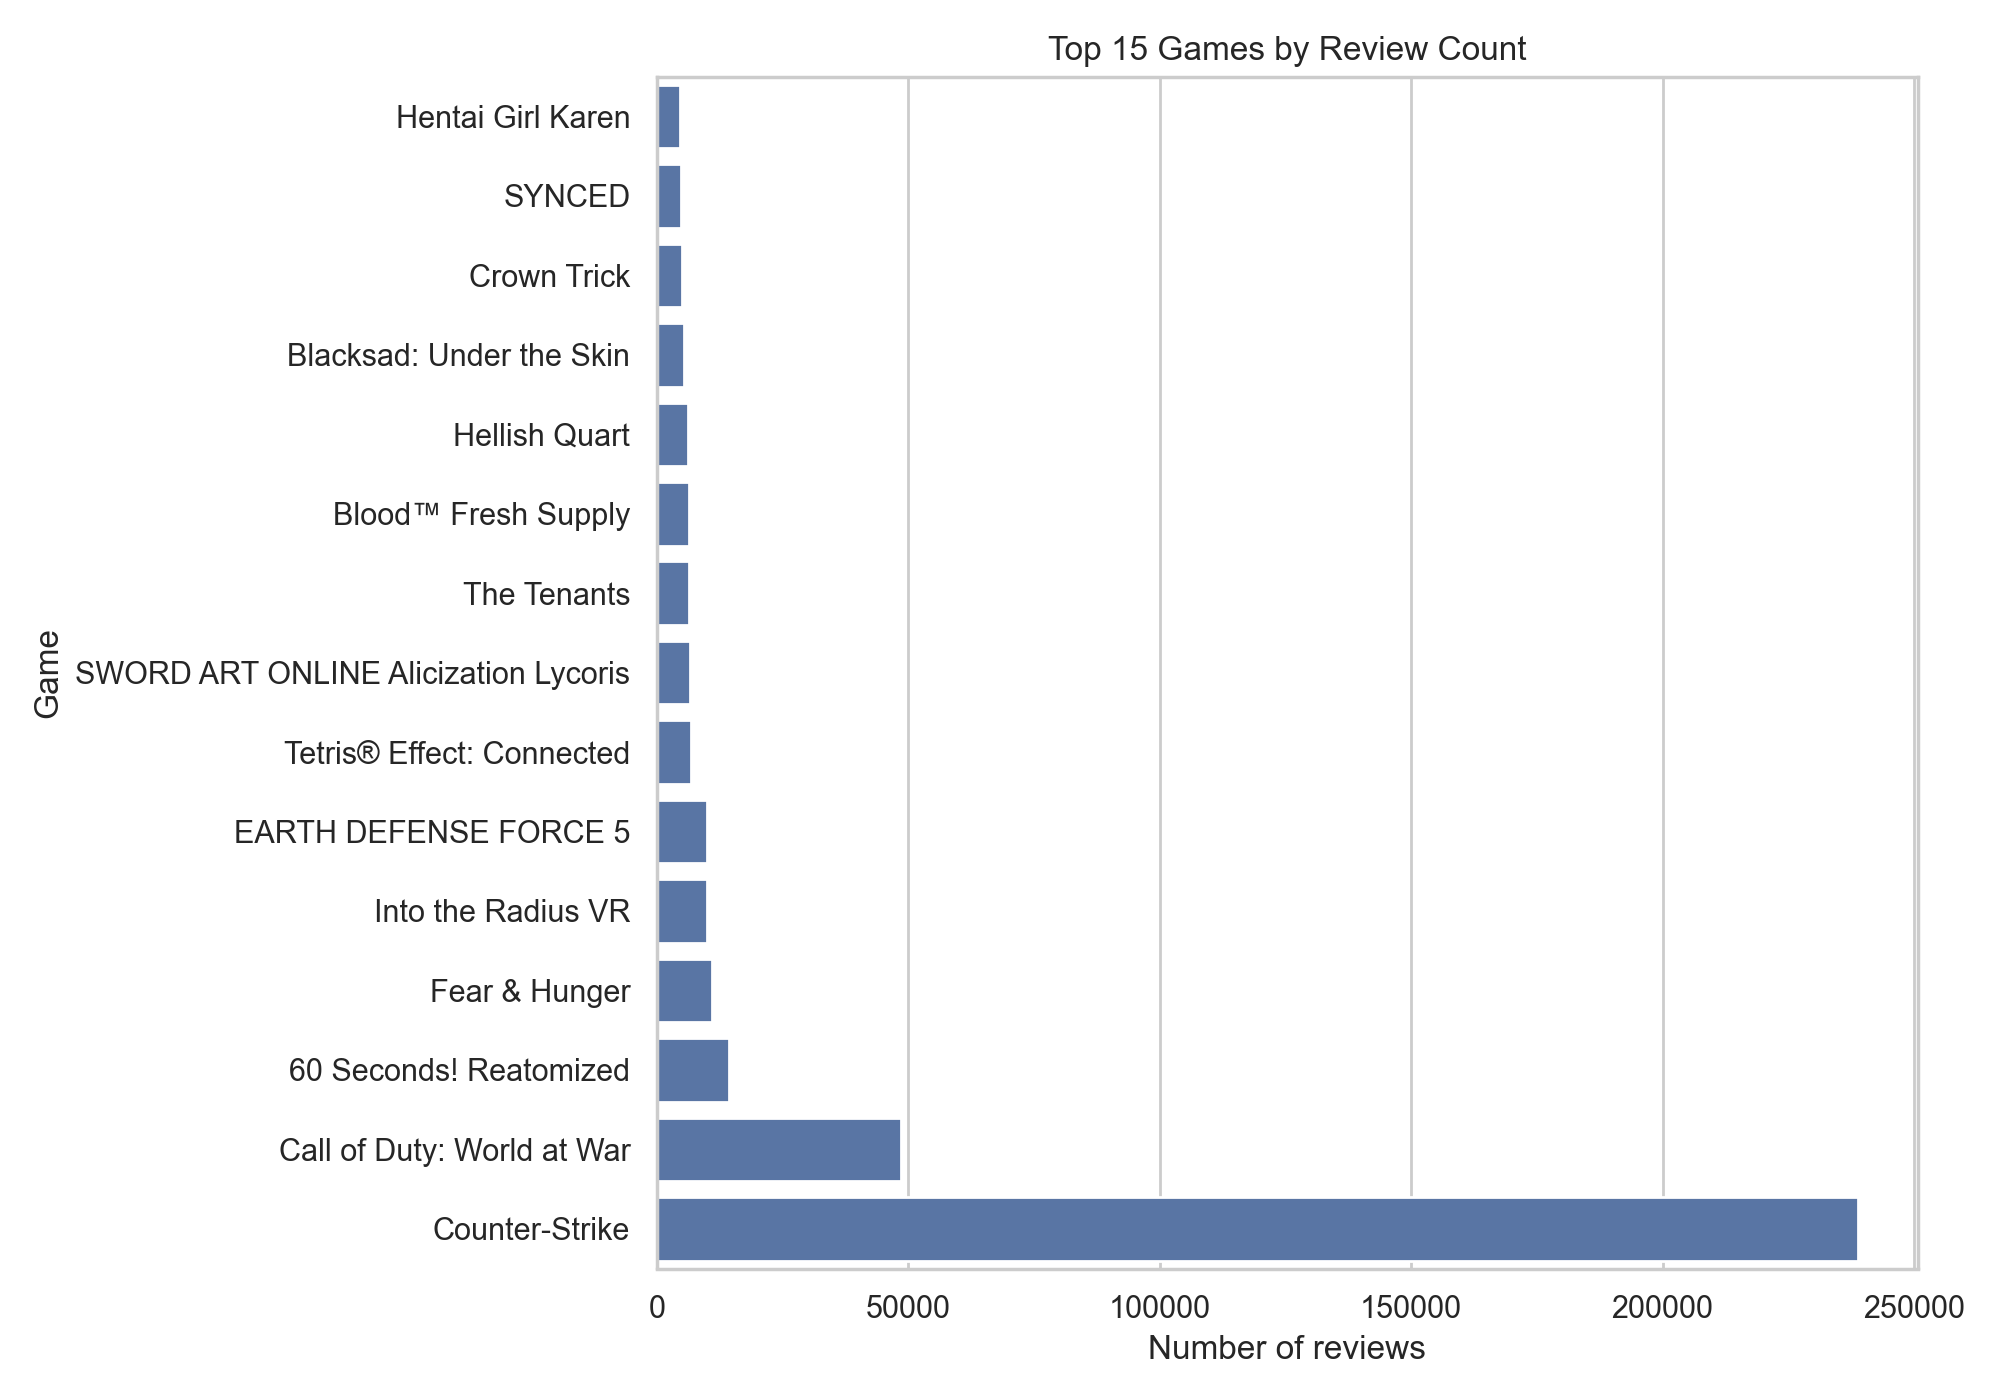
\includegraphics[width=0.9\linewidth]{eda/03_top_games_by_reviews.png}
  \caption{Top games ranked by number of review records in the V1 subset.}
\end{figure}

\subsection*{4) Recommendation Rate for Top Games}
This figure compares satisfaction proxy (recommendation rate) among the most-reviewed titles. It separates high-volume games that are broadly well received from those with mixed sentiment. Because this metric is conditional on sample coverage, values should be interpreted as preliminary and re-estimated on larger or full data before product decisions.

\begin{figure}[H]
  \centering
  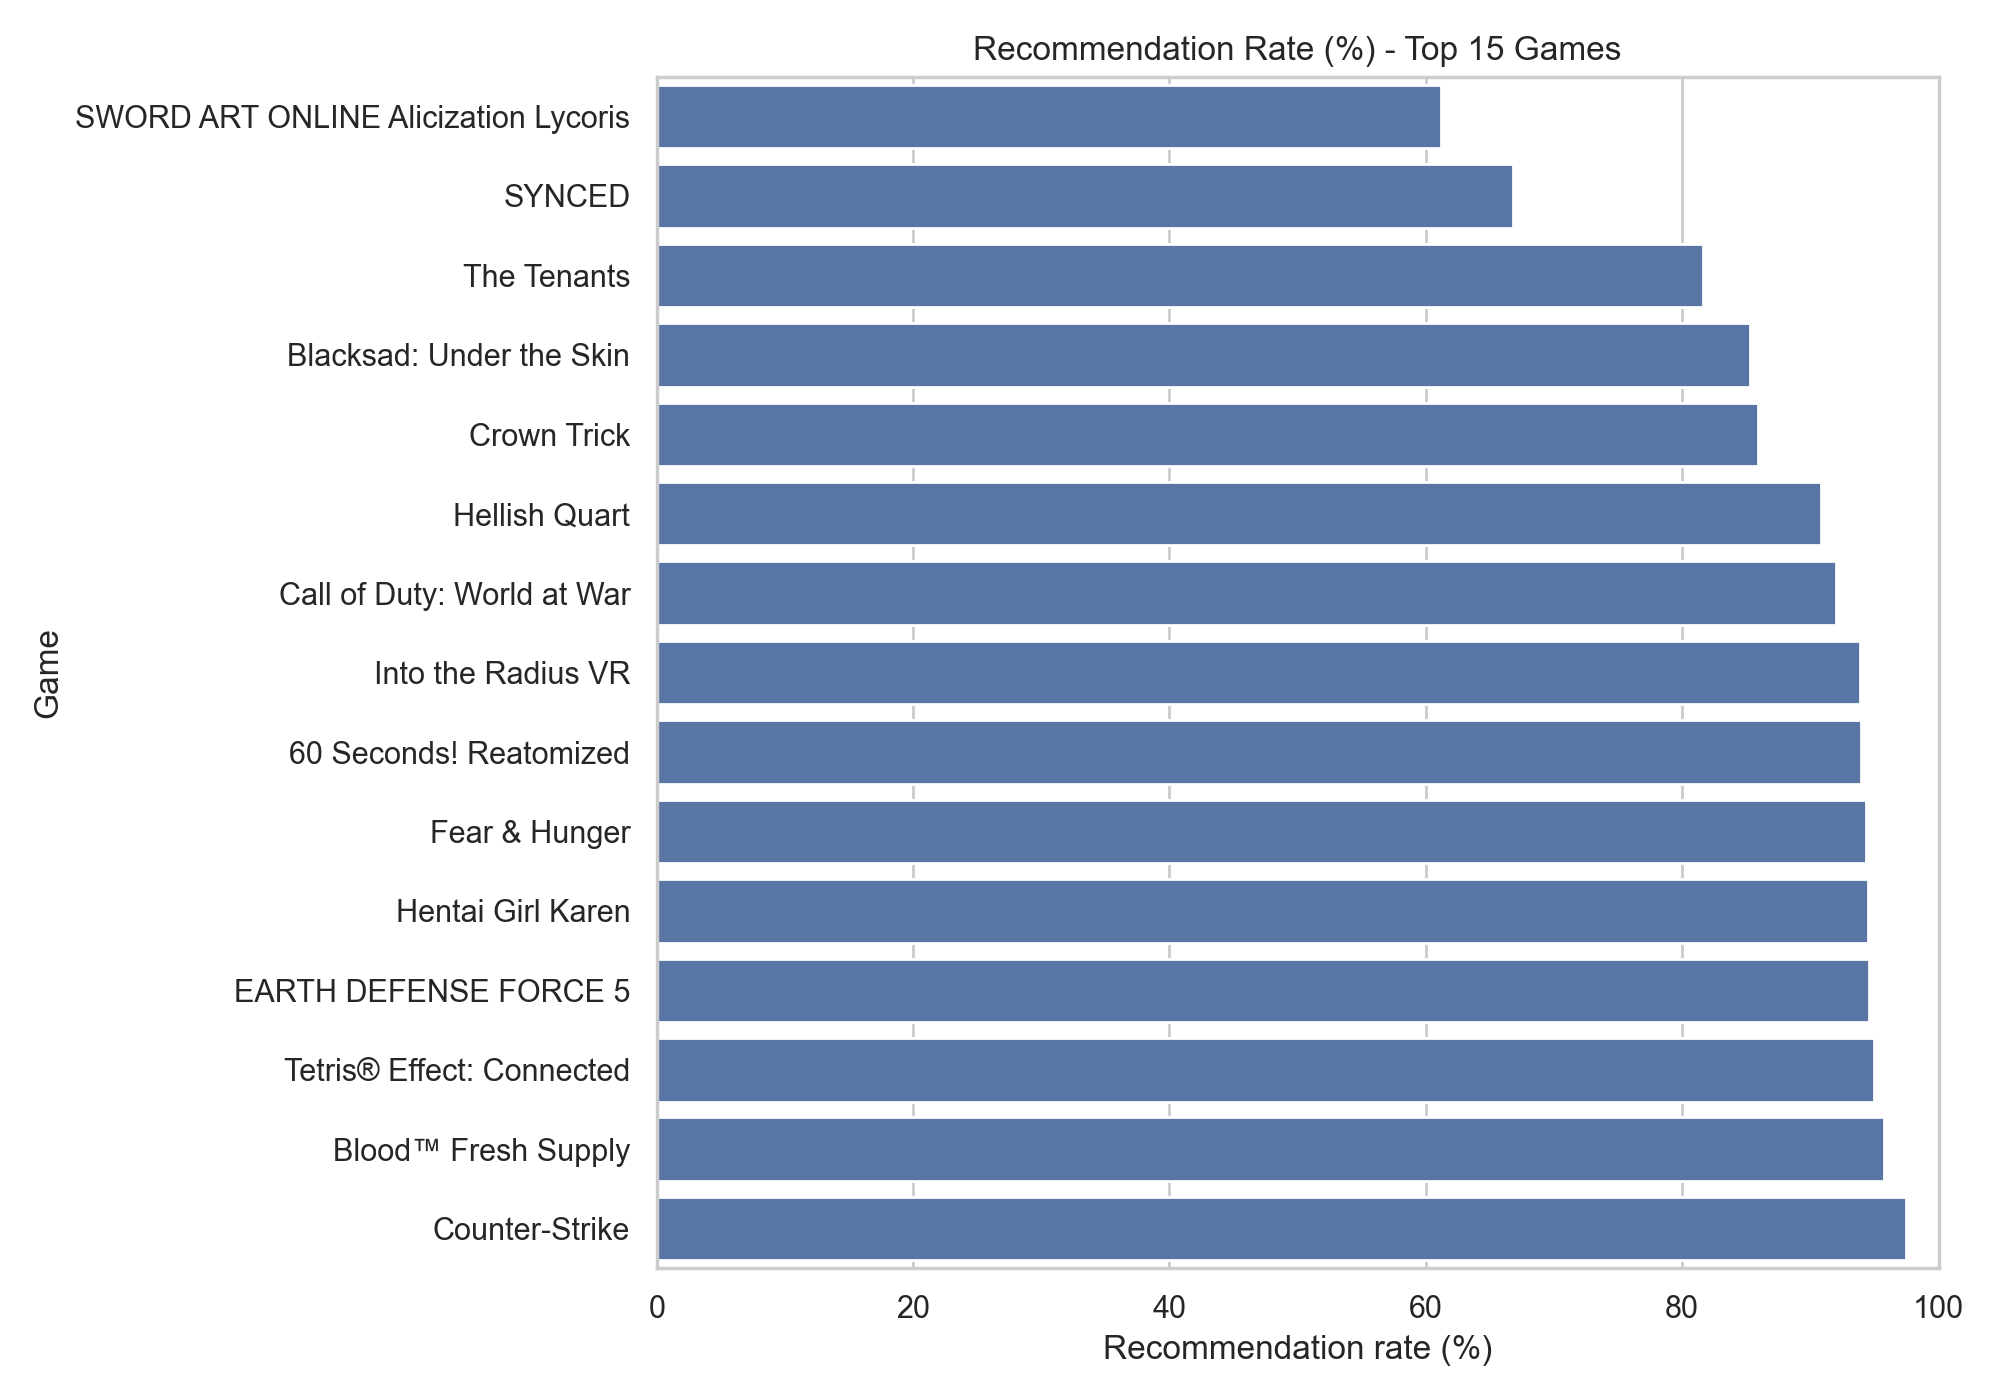
\includegraphics[width=0.9\linewidth]{eda/04_recommendation_rate_top_games.png}
  \caption{Recommendation rate (\%) among games with the highest review volume.}
\end{figure}

\subsection*{5) Top Genres by Review Volume}
This chart highlights which genres dominate observed interaction activity after joining review and catalog data. It helps prioritize segment-level modeling and feature engineering by genre density. Genre rankings may move as the subset changes, but they still provide an initial signal of market attention in the sampled data.

\begin{figure}[H]
  \centering
  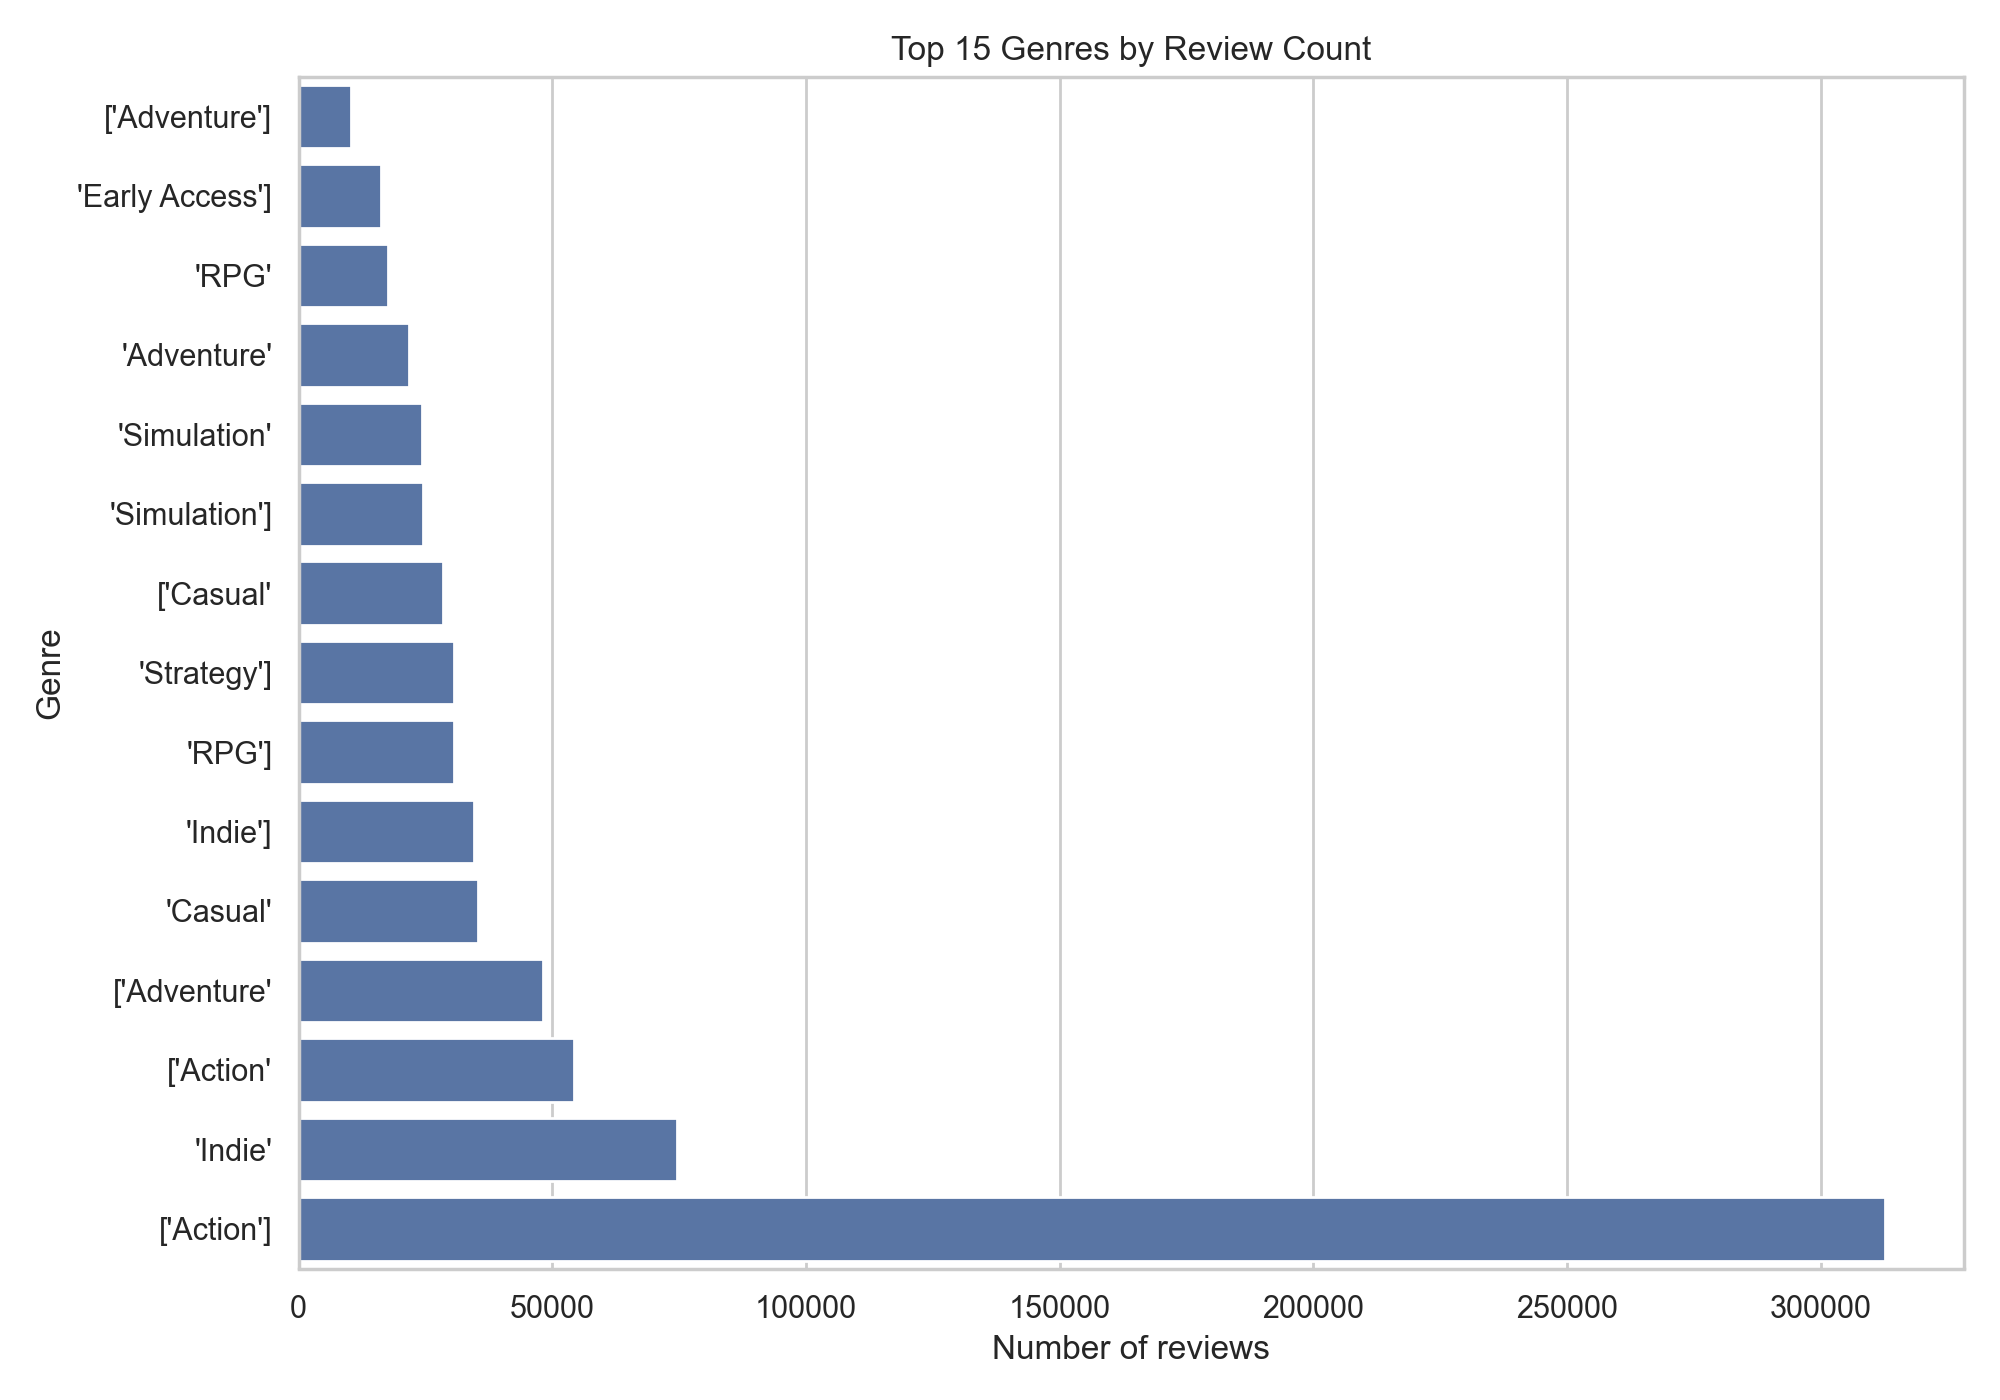
\includegraphics[width=0.9\linewidth]{eda/05_top_genres.png}
  \caption{Most frequent genres in the interaction dataset after catalog join.}
\end{figure}


\end{document}
